\documentclass[a4paper]{article}
\usepackage[margin=1in]{geometry}
\usepackage{amsmath}
\usepackage{graphicx}
\usepackage{subfigure}
\usepackage{indentfirst}
\setlength{\parindent}{0cm}
\usepackage{bm}


\begin{document}
\title{Report on Programme Assignment 1\footnotemark[1]}
\author{Liu Ziquan\\ 54874777}
\footnotetext[1]{The programme language I use is Python. \emph{cvxopt}, \emph{numpy} and \emph{matplotlib} are used in the programme.}
\maketitle
\section{Polynomial function}
\subsection{Task a}
For least-squres, Bayesian and regularized least-squres regression, there are closed-form expression for parameters. But in LASSO and robust regression, we need to adopt concex optimization techniques to get a solution. Initial forms of the two optimization problems cannot be solved by linear programming or quadratic programming so we need to transform the problems into linear programming and quadratic programming.\\
\\
First, we give the quadratic form of LASSO. The original problem of LASSO is
\begin{equation}
  \min_{\theta}\| y-\Phi^T\theta \|^2+\lambda \| \theta \|_1
\end{equation}
Since $y$ is a constant with respect to $\theta$, we can expand the $L_2$ norm and write the optimization problem as
\begin{equation}
  \min_{\theta} \theta^TQ\theta+c^T\theta+\lambda \| \theta \|_1
\end{equation}
where $Q=\Phi \Phi^T$ and $c^T=-2y^T\Phi^T$. The $\| \theta \|_1$ is $L_1$ norm which means sum of absolute values of elements of $\theta$. To obtain $L_1$ norm of $\theta$, we assume 2 variables $\theta^+$ and $\theta^-$, s.t.
\begin{equation}
  \theta^+_i=\frac{|\theta_i|+\theta_i}{2},
  \theta^-_i=\frac{|\theta_i|-\theta_i}{2}
\end{equation}
So both $ \theta^+_i$ and $ \theta^-_i$ are non-negative numbers and $ \theta^+_i+ \theta^-_i=|\theta_i|$. In this way, we can eliminate absolute values in the objective function. But at the same time, we will add constraints on the decision variables. The original optimization problem of LASSO can be written as the following form:
\begin{equation}
  \begin{aligned}
  \min_{\bm{x}} \bm{x}^T \bm{H} \bm{x}+\bm{f}^T \bm{x}\\
  s.t. \quad \bm{G}\bm{x}\leq \bm{S}
  \end{aligned}
\end{equation}
where $\bm{x}=$ $\begin{bmatrix} \begin{smallmatrix} \theta^+ \\ \theta^- \end{smallmatrix} \end{bmatrix}$, $\bm{H}=$ $\begin{bmatrix} \begin{smallmatrix} Q & -Q \\ -Q & Q \end{smallmatrix} \end{bmatrix}$, $\bm{f}^T=$ $\begin{bmatrix} \begin{smallmatrix} c^T & -c^T \end{smallmatrix} \end{bmatrix}$. The inequality constraints ensure that $\theta^+_i,\theta^-_i \geq 0$ and $\theta_i<S_i$, where
$\begin{bmatrix} \begin{smallmatrix} I_D & I_D \\ -I_{2D}\end{smallmatrix} \end{bmatrix}$, $S= \begin{bmatrix} \begin{smallmatrix} \bm{s}_D \\ \bm{0}_{2D}\end{smallmatrix}\end{bmatrix}$. This is a QP problem that can be solved by standard QP solver. The hyperparameter is $s$ instead of $\lambda$.\\
\\
Now we transform robust regression to LP form. $|y_i-\phi^T_i\theta |\leq u_i$ is equivalent to $-u_i\leq y_i-\phi^T_i\theta \leq u_i$. So the original problem can be written as
\begin{equation}
  \begin{aligned}
    \min_{\bm{x}} [\bm{1}_n^T \quad \bm{0}_D^T]\bm{x}\\
    s.t. \quad \bm{P}\bm{x}\leq \bm{Y}
  \end{aligned}
\end{equation}
where $\bm{x} =\begin{bmatrix} \begin{smallmatrix} u \\ \theta \end{smallmatrix} \end{bmatrix}$, $\bm{P}=\begin{bmatrix} \begin{smallmatrix} -I_n & \Phi^T \\ -I_n & -\Phi^T \end{smallmatrix} \end{bmatrix}$ and  $\bm{Y} =\begin{bmatrix} \begin{smallmatrix} y \\ -y \end{smallmatrix} \end{bmatrix}$. This is a LP problem that can be sovled by standard LP solver. 


\subsection{Task b}
In this part, we test the 5 regression algorithms written in Task a. Through testing different hyperparameters in BR, LASSO and regularized LS, we adopt hyperparameters as $\alpha = 1$, $s=1$, $\lambda = 1.8$. We train the regression algotirhms on sample data and test on true data. Figure \ref{f_1b} depicts training and testing result. For BR, standard deviation is plotted as errorbar. The prediction line of LSE and Lasso overlap with the true function line to a large extent. But RR, BR and regularized SE do not overlap with the true function line so perfectly.\\

\begin{figure}[h]
  \centering
  \includegraphics[width=.3\textwidth]{Task_b/LSE}
  \includegraphics[width=.3\textwidth]{Task_b/Rob}
  \includegraphics[width=.3\textwidth]{Task_b/Rgl}
  \includegraphics[width=.3\textwidth]{Task_b/BayesRegression}
  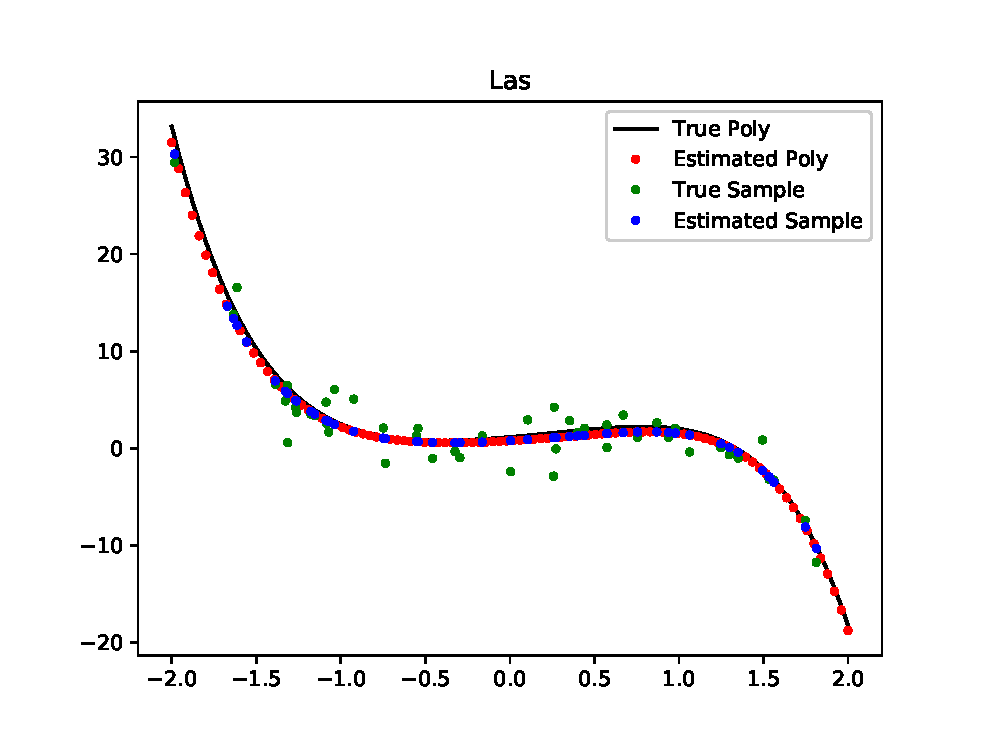
\includegraphics[width=.3\textwidth]{Task_b/Las}
  \caption{Regression Result of Task b}
  \label{f_1b}
\end{figure}

The mean-squared error(MSE) of 5 algorithms on the test set is shown in Table \ref{table1}. From the mean-squared error, we can see that Lasso performs best in the 5 algorithms. Robust regression has the lowest accuracy. But RR is the most robust one to outliers, which will be shown in next section.  LSE, regularized SE and BR have the same level of accuracy.
\begin{table}[h]
  \centering
\begin{tabular}{|c|c|c|c|c|}
  \hline
  RR & LSE &Regularized SE & BR& Lasso \\
  \hline
  0.7680&0.4086&0.3916&0.4592&0.3596 \\
  \hline
\end{tabular}
\caption{Predict Error on Test Set}
\label{table1}
\end{table}


\subsection{Task c}
In this section, we change the size of training set to see which algorithm tends to overfit. First, we sample data randomly from the whole training set, whose size is 50 data points, to generate 4 subsets with 6, 10, 20 and 30 data points respectively. Like in Task b, we plot their results on testing set in Figure \ref{f_6_points}-\ref{f_30_points}. When training on 6 and 10 points, estimate functions of LSE and RR are far from true function, which means LSE and RR are not robust with less data. BR, regularized SE and Lasso perform well on less data, which means the 3 methods are robust to insufficient data.\\
\\
The above result is obtained through once random sample from original data so the result includes random factors. To get more stable result, we run random sample 5000 times at each subset size from 8 data points to 50 data points and plot mean-squared error(MSE) versus training size in Figure \ref{f_error_ds}. LSE and RR have the same feature: when training size is small, prediction error is very large while when training size reaches a certain amount, prediction error will become relatively small. BR is the most accurate algorithm among the 5 when training on a small data set. Regularized SE has the same accurate level as BR but a little worse. Lasso's error is larger than BR and regularized SE on less training data. But when training size becomes larger, Lasso's accuracy improves faster than BR and regularized SE.
\begin{figure}[h]
  \centering
  \includegraphics[width=.25\textwidth]{6/6_LSE}
  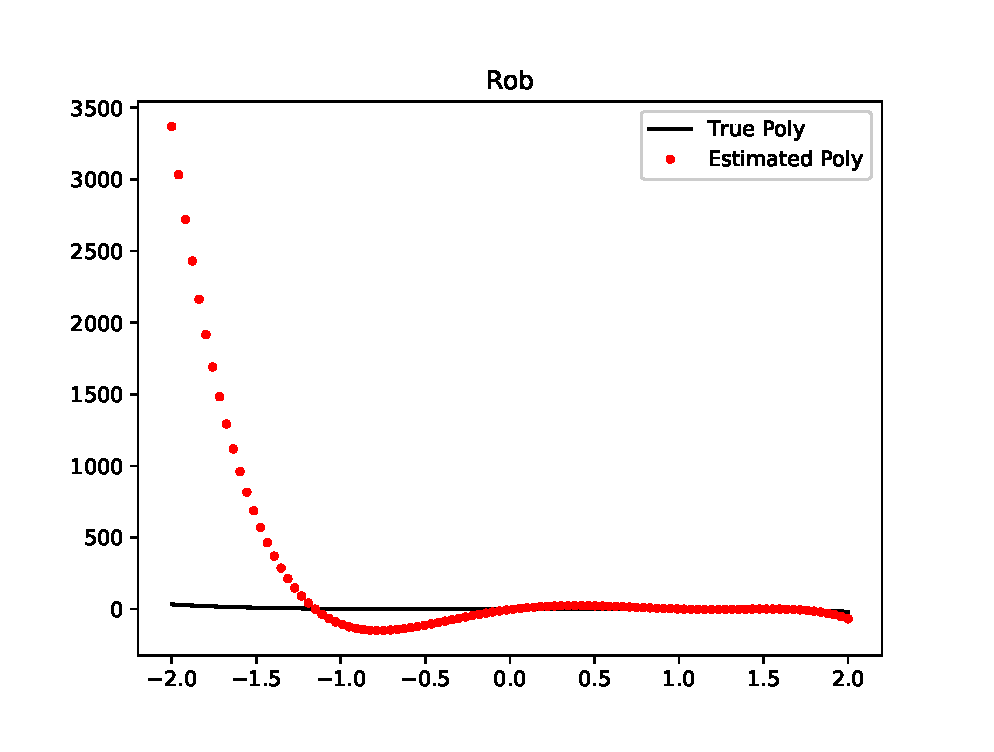
\includegraphics[width=.25\textwidth]{6/6_Rob}
  \includegraphics[width=.25\textwidth]{6/6_Rgl}
  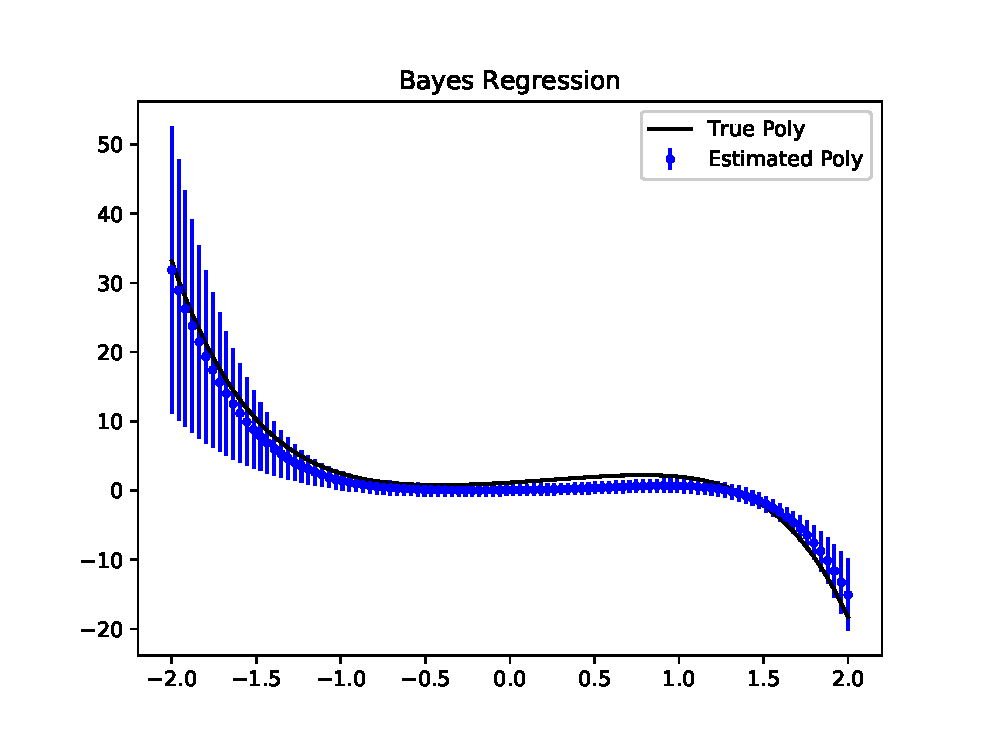
\includegraphics[width=.25\textwidth]{6/6_BayesRegression}
  \includegraphics[width=.25\textwidth]{6/6_Las}
  \caption{Training on 6 points}
  \label{f_6_points}
\end{figure}
\begin{figure}[h]
  \centering
  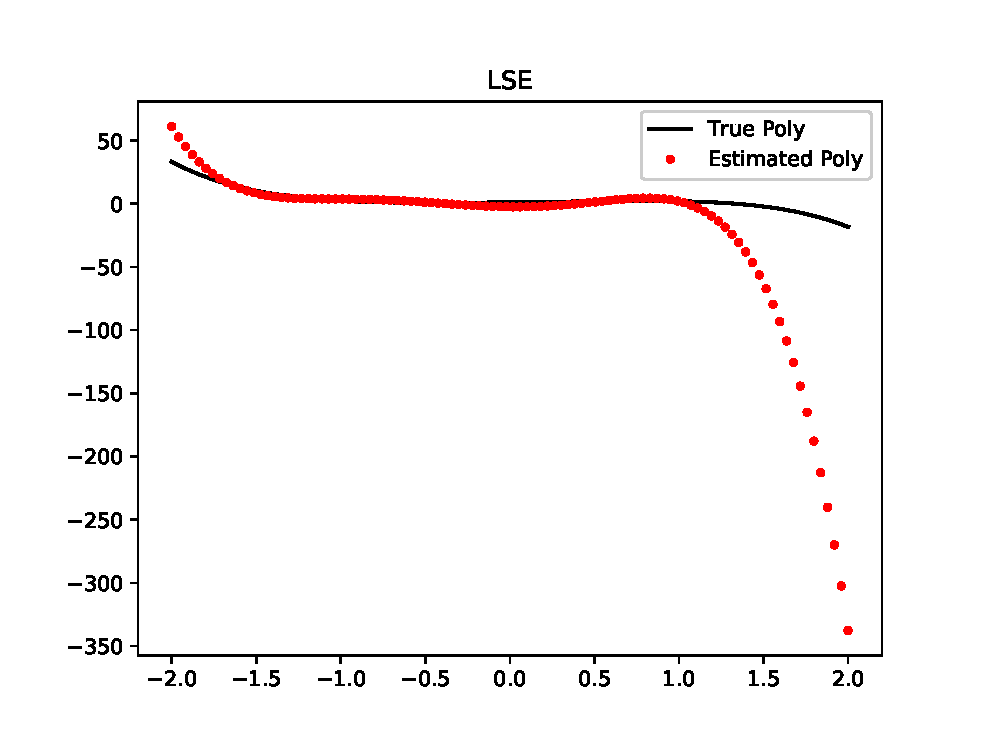
\includegraphics[width=.25\textwidth]{10/10_LSE}
  \includegraphics[width=.25\textwidth]{10/10_Rob}
  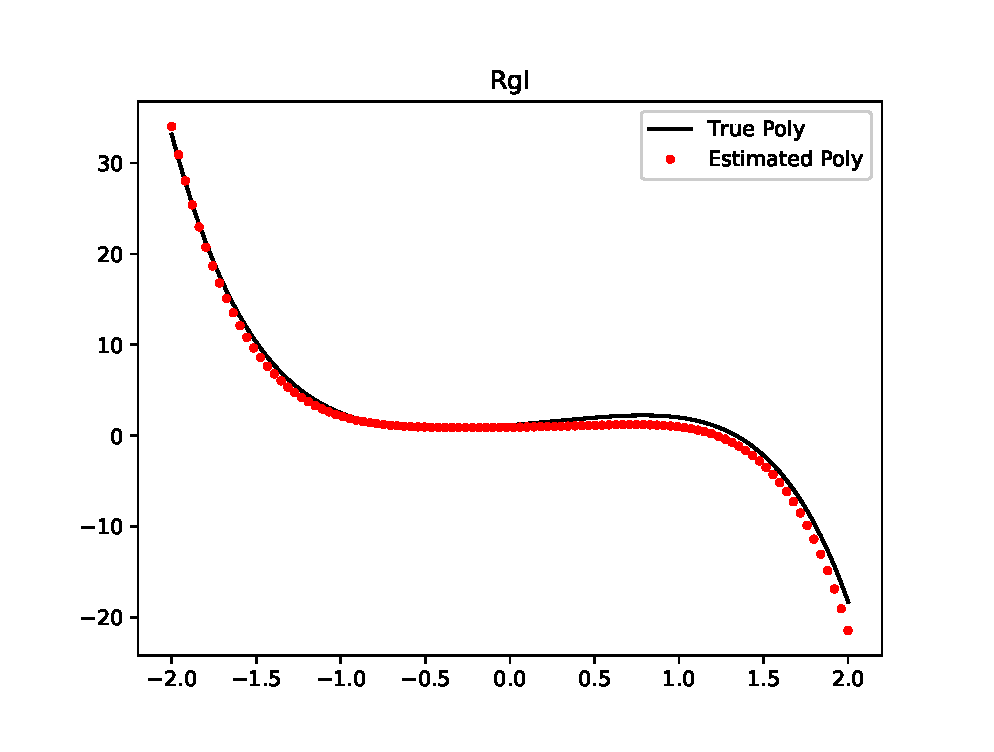
\includegraphics[width=.25\textwidth]{10/10_Rgl}
  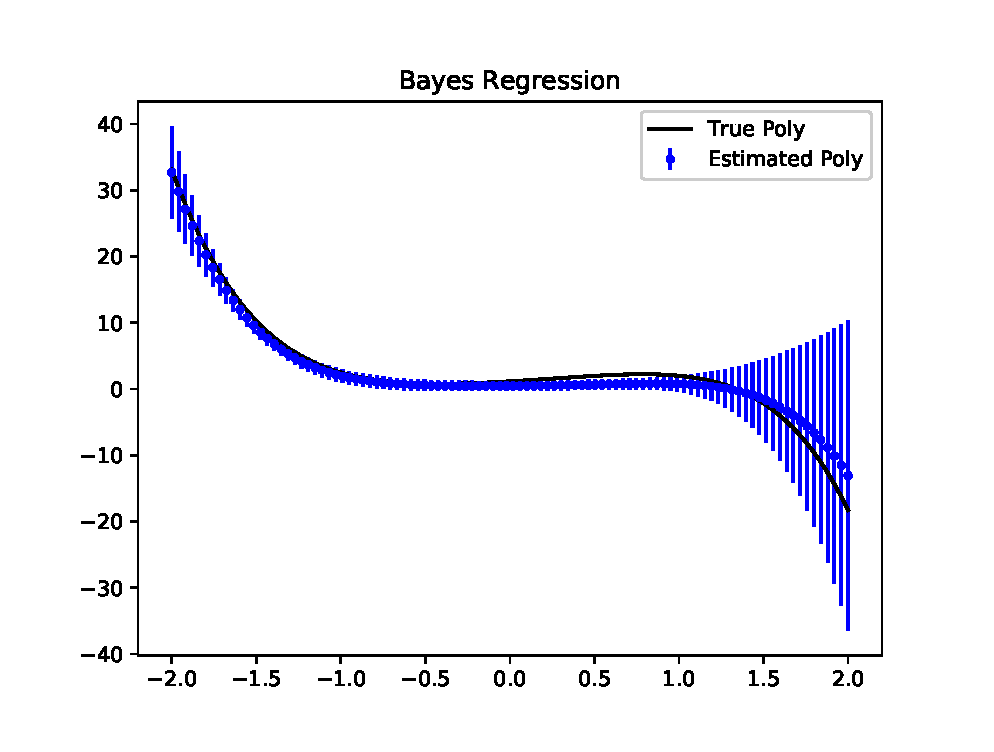
\includegraphics[width=.25\textwidth]{10/10_BayesRegression}
  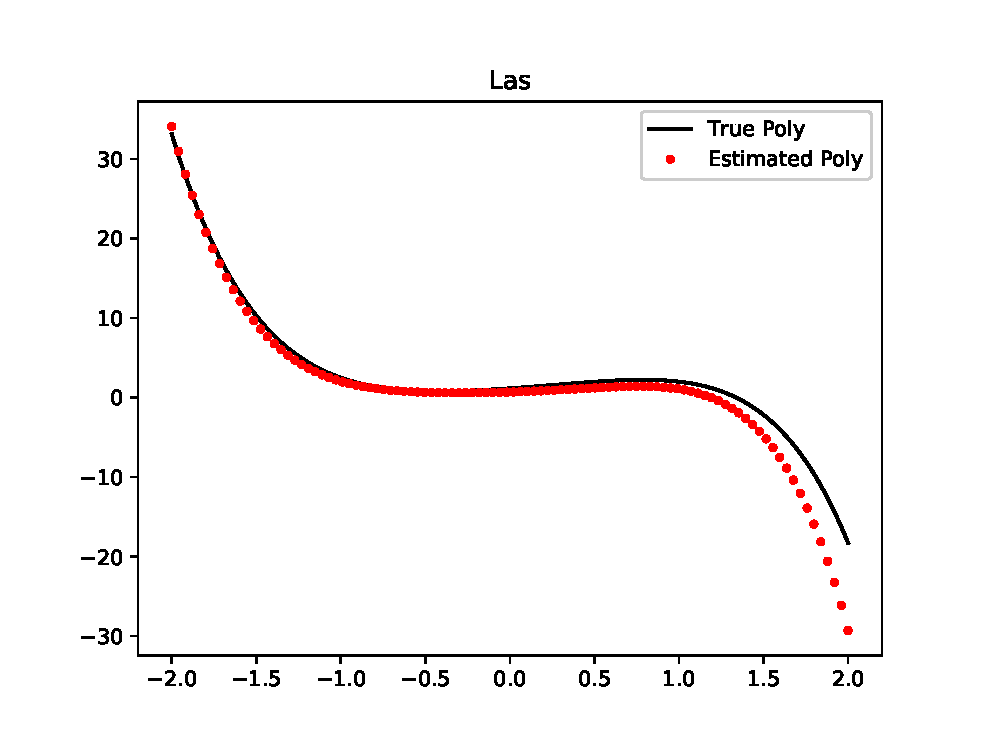
\includegraphics[width=.25\textwidth]{10/10_Las}
  \caption{Training on 10 points}
  \label{f_10_points}
\end{figure}
\begin{figure}[h]
  \centering
  \includegraphics[width=.25\textwidth]{20/20_LSE}
  \includegraphics[width=.25\textwidth]{20/20_Rob}
  \includegraphics[width=.25\textwidth]{20/20_Rgl}
  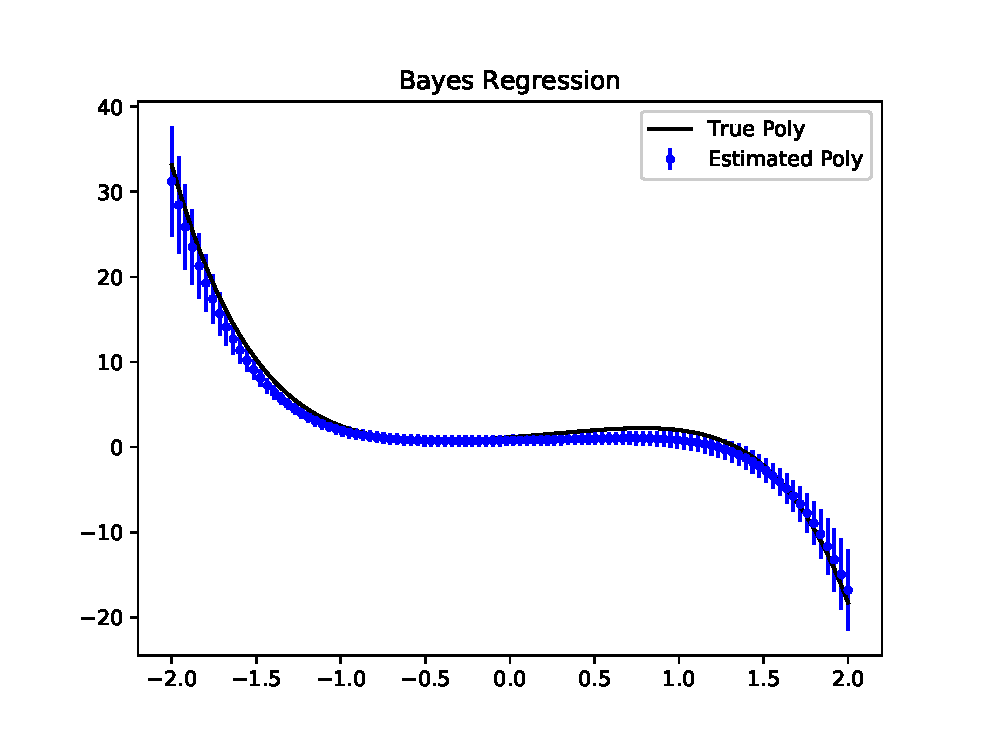
\includegraphics[width=.25\textwidth]{20/20_BayesRegression}
  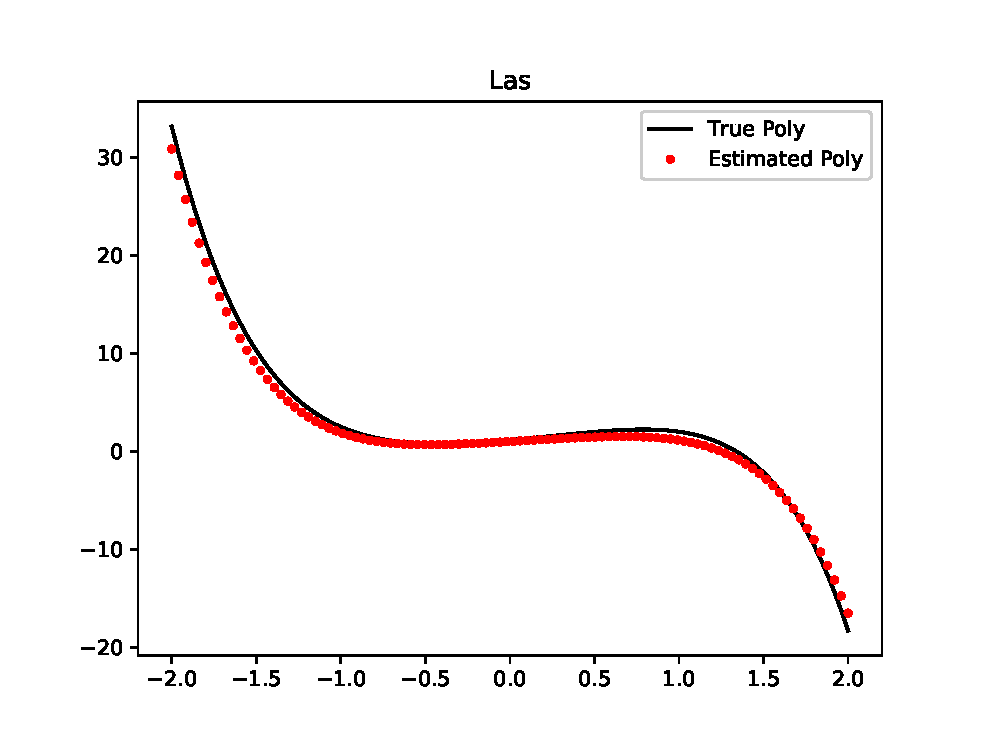
\includegraphics[width=.25\textwidth]{20/20_Las}
  \caption{Training on 20 points}
  \label{f_20_points}
\end{figure}
\begin{figure}[h]
  \centering
  \includegraphics[width=.25\textwidth]{30/30_LSE}
  \includegraphics[width=.25\textwidth]{30/30_Rob}
  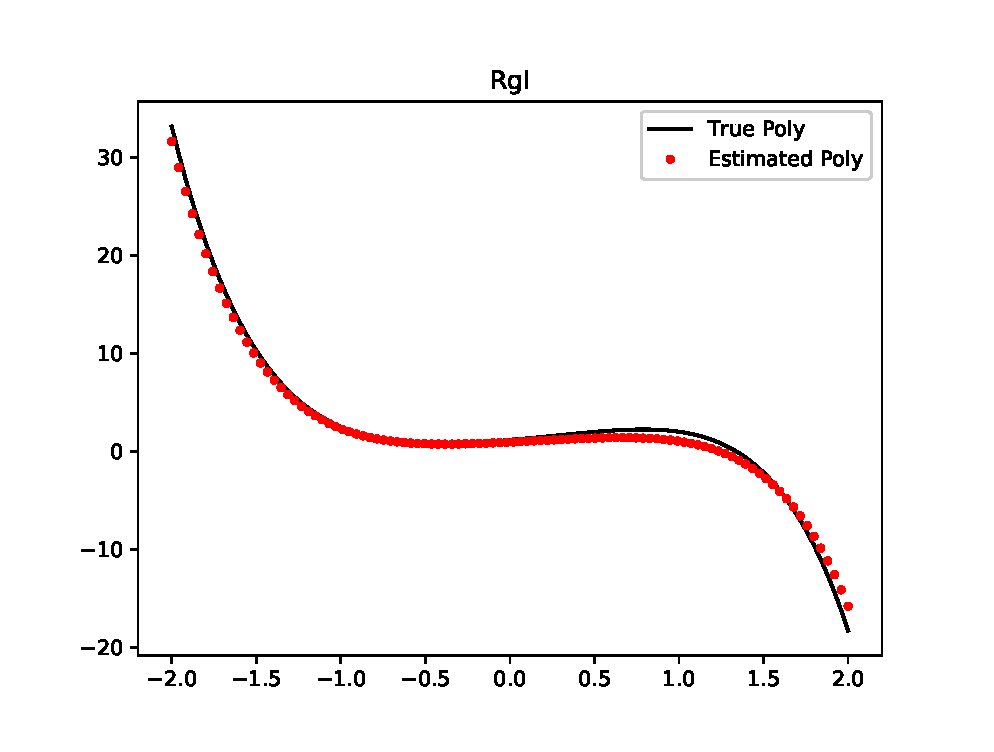
\includegraphics[width=.25\textwidth]{30/30_Rgl}
  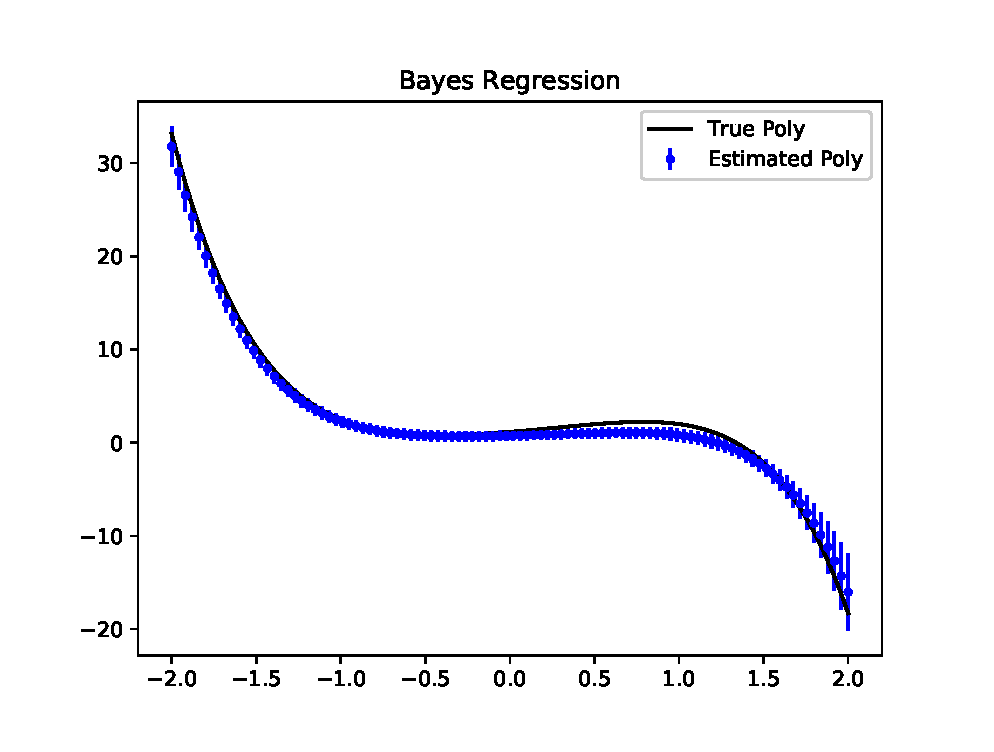
\includegraphics[width=.25\textwidth]{30/30_BayesRegression}
  \includegraphics[width=.25\textwidth]{30/30_Las}
  \caption{Training on 30 points}
  \label{f_30_points}
\end{figure}
\begin{figure}[h]
  \centering
  \includegraphics[width=.25\textwidth]{Ave/LSE}
  \includegraphics[width=.25\textwidth]{Ave/Robust}
  \includegraphics[width=.25\textwidth]{Ave/Rgl}
  \includegraphics[width=.25\textwidth]{Ave/Bayes}
  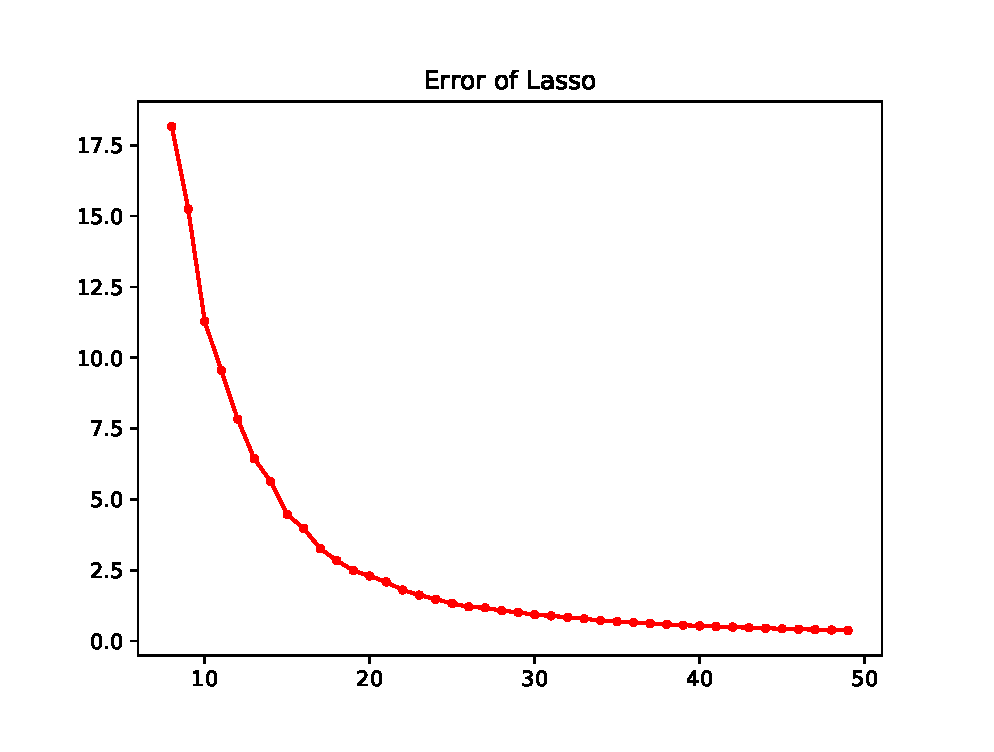
\includegraphics[width=.25\textwidth]{Ave/Lasso}
  \caption{Error vs. training data size}
  \label{f_error_ds}
\end{figure}
\clearpage
\subsection{Task d}
In this section, we set some outliers to the training set to test robustness of regression algorithms to abnormal values. In the experiment, we randomly select 5 data points from training set and set their $y$ values to be randomly large compared to normal sample values. The result is shown in Figure \ref{f_d}. MSE of each model is also given in figures\\
\\
The result shows that LSE, regularized SE and Bayes Regression are all very sensitive to outliers since there are no overlap between estimate function and true function. The most sensitive algorithm is LSE. Estimate function of Lasso has a small region which is overlapped with true function. RR is the most robust algorithm to outliers among the 5 methods. The reason for robustness of RR is that when there are abnormal values in training set, the residual is measured by $L_1$ norm, which makes it less sensitive to large residuals compared to $L_2$ norm. That is why LSE is most sensitive to outliers: it only tends to minimize $L_2$ norm of residual, which is very large when there are outliers in training set. When the residual of outliers is large, it will affact the optimization result to a very large extent. 
\begin{figure}[h]
  \centering
  \includegraphics[width=.25\textwidth]{Task_d/LSE}
  \includegraphics[width=.25\textwidth]{Task_d/Rob}
  \includegraphics[width=.25\textwidth]{Task_d/Rgl}
  \includegraphics[width=.25\textwidth]{Task_d/BayesRegression}
  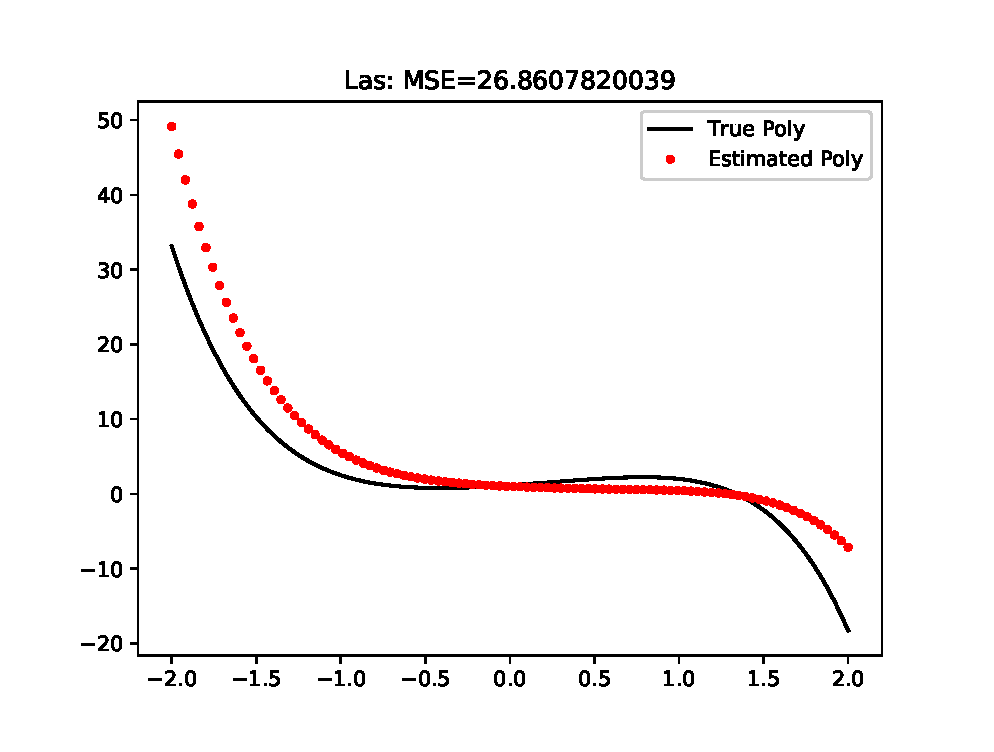
\includegraphics[width=.25\textwidth]{Task_d/Las}
  \caption{Result on Training Set with Anomaly}
  \label{f_d}
\end{figure}

\subsection{Task e}
Task e is to try high-order polynomial to model the function and to see which algorithm is more prone to overfitting. To do this task, we just need to change the dimension of feature and perform regression. We obtain the following result when using 10th order polynomial in Figure \ref{f_e}. Both prediction function and MSE are give in the figure. Lasso is the worst algorithm considering its largest MSE. But the estimate function of Lasso is not complex because of its regularization term. Regularized SE and BR also learned less complex functions than LSE and RR because of regularization and their MSEs are at the middle level. Both LSE and RR learned complex functions but LSE's MSE is much larger than RR's, which shows RR's robustness to complex model.
\clearpage
\begin{figure}[h]
  \centering
  \includegraphics[width=.25\textwidth]{Task_e/LSE}
  \includegraphics[width=.25\textwidth]{Task_e/Rob}
  \includegraphics[width=.25\textwidth]{Task_e/Rgl}
  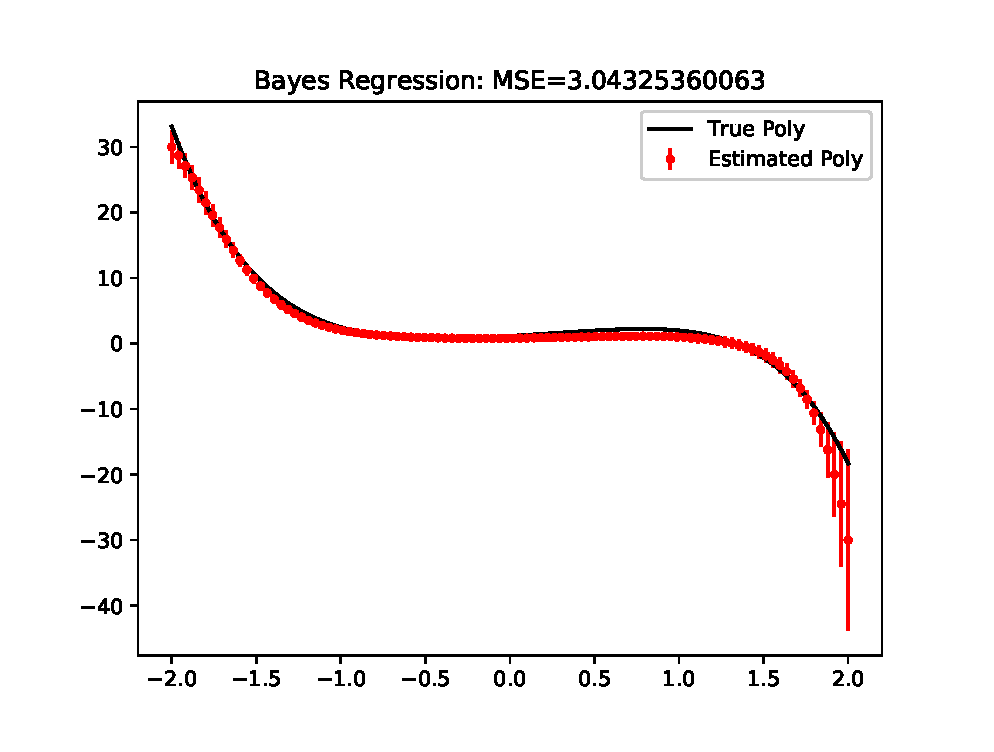
\includegraphics[width=.25\textwidth]{Task_e/BayesRegression}
  \includegraphics[width=.25\textwidth]{Task_e/Las}
  \caption{Result of 10th order}
  \label{f_e}
\end{figure}

\section{Counting People}
Based on regression model in Part 1, we learn a regression function and predict number of people in an image. Since we already have regression codes, we can directly use the 'Regressor' class to do regression in this part.
\subsection{Task a}
We set feature $\phi (x)=x$ and do regression using the above 5 models. Then test the regression function on test set, we compare the predicion values and true values in Figure \ref{f_counting1}. MSE and MAE of each algorithm are also given in the figure. From MSE and MAE result, we can see that regularized SE works best among the 5 methods. BR is a little worse than regularized SE. LSE and RR's accuracies are at the same level. Lasso's accuracy is the lowest one. 
\begin{figure}[h]
  \centering
  \includegraphics[width=.25\textwidth]{Counting1/LSE}
  \includegraphics[width=.25\textwidth]{Counting1/Rob}
  \includegraphics[width=.25\textwidth]{Counting1/Rgl}
  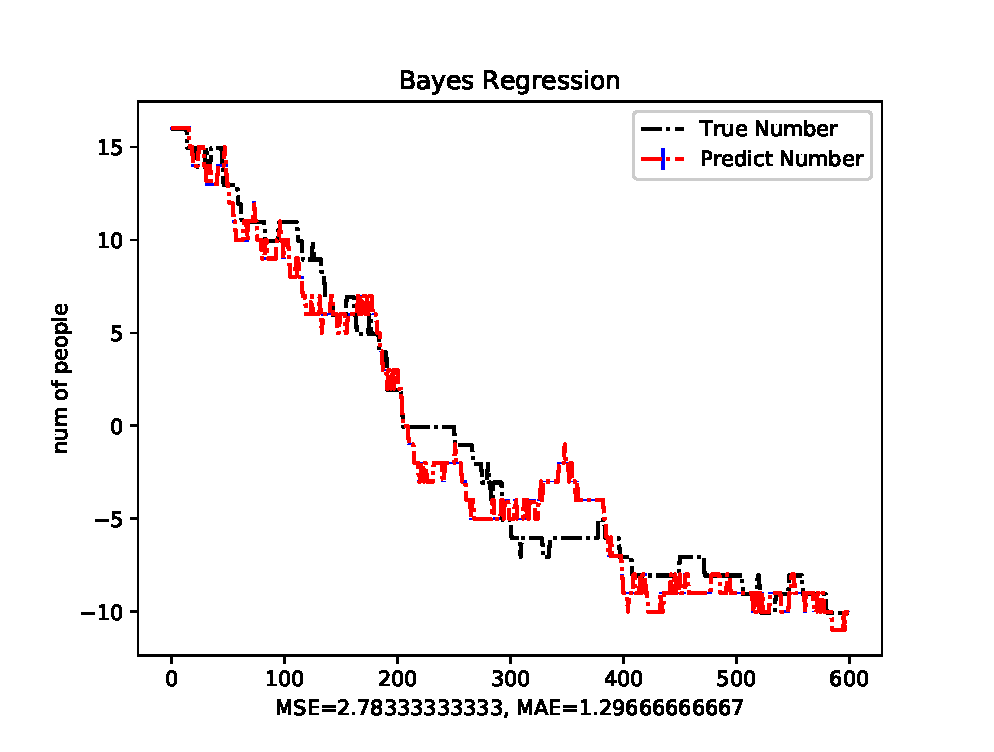
\includegraphics[width=.25\textwidth]{Counting1/BayesRegression}
  \includegraphics[width=.25\textwidth]{Counting1/Las}
  \caption{Prediction and True Counting Using $x$ as Feature}
  \label{f_counting1}
\end{figure}


\subsection{Task b}
In this task, we use different features to do regression. Specifically, we use 2nd and 3rd order polynomial as features, i.e. $\phi (x)=[x_1,\dots,x_9,x_1^2,\dots,x_9^2]^T$ and  $\phi (x)=[x_1,\dots,x_9,x_1^2,\dots,x_9^2,x_1^3,\dots,x_9^3]^T$. Results of the two features are shown in Figure \ref{f_counting2_1} and \ref{f_counting2_2}. We also try add some cross-terms $x_ix_j$ but the result is not improved but degenerates, so we do not give cross-term feature's result. 2nd order polynomial feature improves all methods' accuracy. But 3rd order polynomial feature does not improve accuracy of 2nd order in terms of RR and BR. Lasso's accuracy is improved largely when using 3rd order polynomial. Regularized SE is always the best approach in this task. 
\begin{figure}[h]
  \centering
  \includegraphics[width=.25\textwidth]{Counting2_1/LSE}
  \includegraphics[width=.25\textwidth]{Counting2_1/Rob}
  \includegraphics[width=.25\textwidth]{Counting2_1/Rgl}
  \includegraphics[width=.25\textwidth]{Counting2_1/BayesRegression}
  \includegraphics[width=.25\textwidth]{Counting2_1/Las}
  \caption{Prediction and True Counting Using 2nd Feature}
  \label{f_counting2_1}
\end{figure}

\begin{figure}[h]
  \centering
  \includegraphics[width=.25\textwidth]{Counting2_2/LSE}
  \includegraphics[width=.25\textwidth]{Counting2_2/Rob}
  \includegraphics[width=.25\textwidth]{Counting2_2/Rgl}
  \includegraphics[width=.25\textwidth]{Counting2_2/BayesRegression}
  \includegraphics[width=.25\textwidth]{Counting2_2/Las}
  \caption{Prediction and True Counting Using 3rd Feature}
  \label{f_counting2_2}
\end{figure}




\end{document}